\chapter[2022 April]{April 2022}

\section[2022/04/01]{Saturday, 02 April 2022}
\label{sec:20220401}

\subsection{Initial prototypes}

A small prototype was built using \href{https://teachablemachine.withgoogle.com}{Teachable Machine} to see if a small neural network could serve as the basis for the hand gesture recognition system if discrete gestures were used. Most of the research papers reviewed so far generate a three-dimensional model of the hand which is likely necessary for fine-grained control of the virtual object and will need to be implemented. But it is also uncertain if the segmentation and explicit hand position calculation approach is going to be necessary given how successful Zhang et.al's deep-learning only approach \cite{mediapipe_hands} to generating a three-dimensional hand model is. \newline

\FigRef{fig:teachablemachine1} shows an open-hand input to the teachable Machine prototype and \FigRef{fig:teachablemachine2} shows the closed-hand input. The two different hand gestures either rotate a cube to it's leftmost face or topmost face. The algorithm works in a web browser and using a webcam for input can accurately rotate the cube based on hand input. Thus, it is relatively trivial to implement discrete gesture recognition using off-the-shelf software like Tensorflow with basic neural networks trained on small amounts of data (less than 1000 images). The prototype is extremely simple and because it is not optimized or trained with lots of data it breaks down when seeing new input - like an open hand but with the user wearing a mask but demonstrates that small neural networks can be used for discrete gesture recognition. \newline

\begin{figure}[!ht]
  \centering
  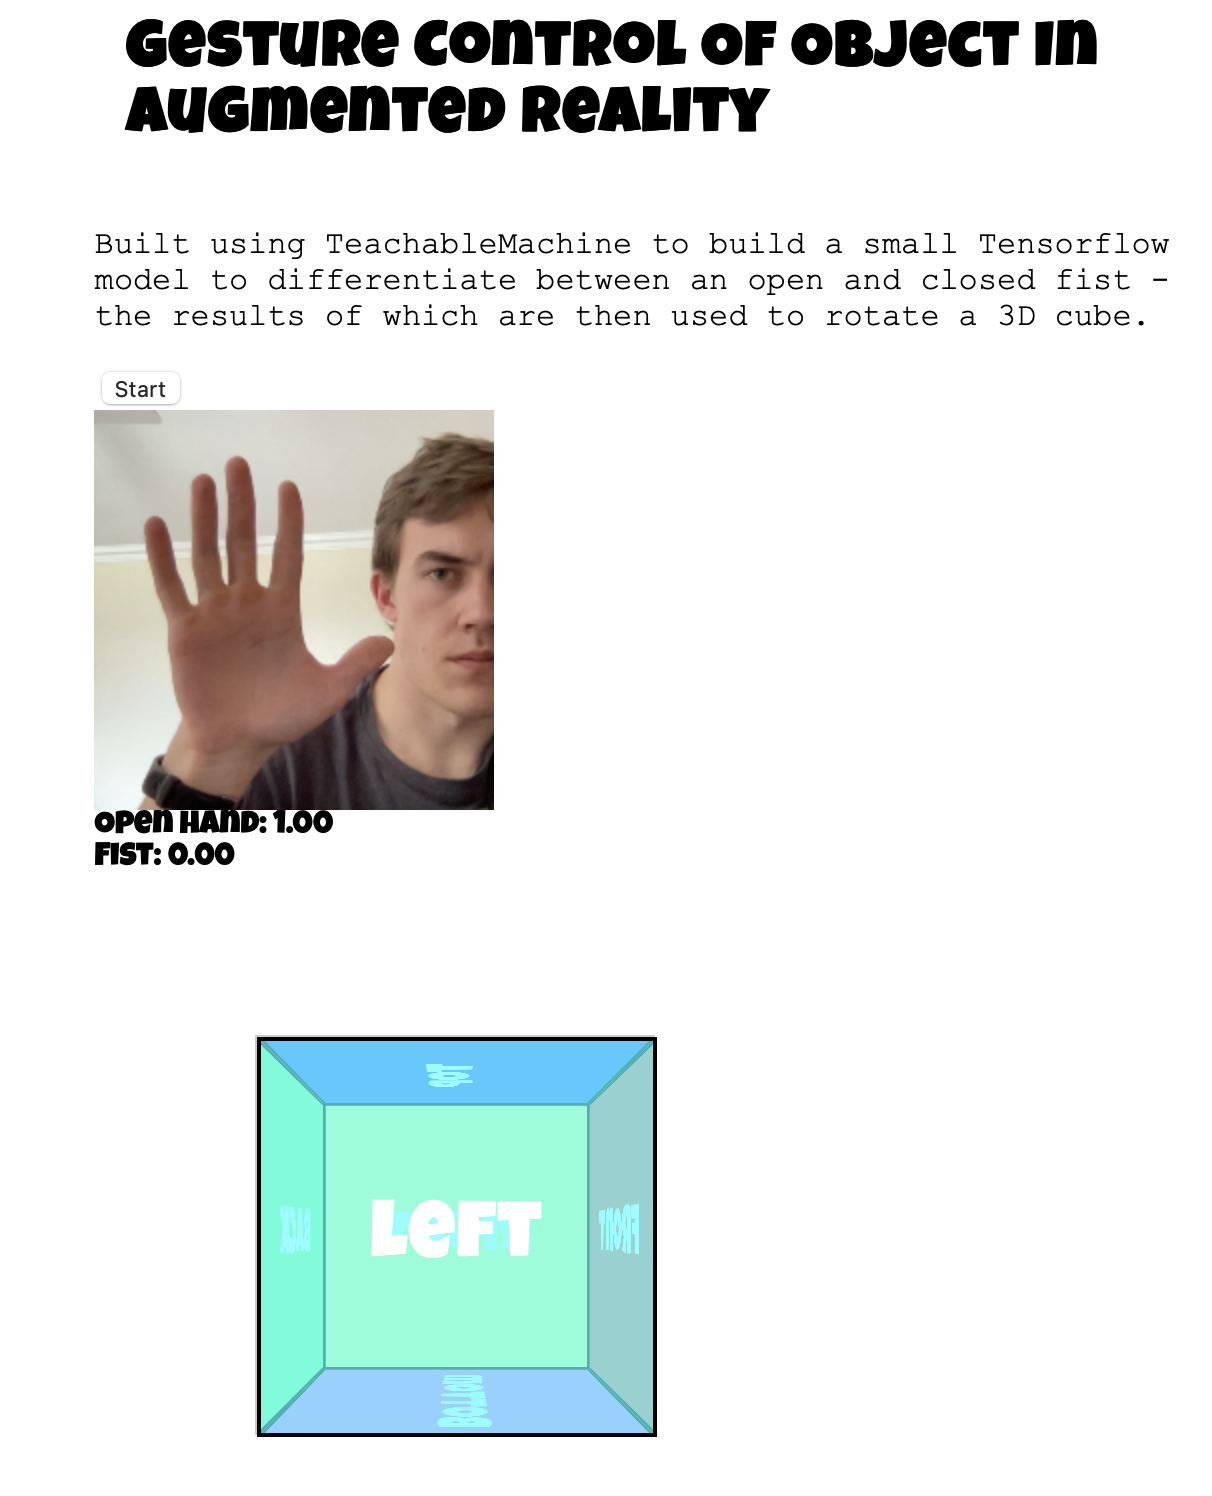
\includegraphics[width=0.4\linewidth]{figures/teachable_machine_1.png}
  \caption{Open-hand input to TeachableMachine gesture recognition prototype}
  \label{fig:teachablemachine1}
\end{figure}
\begin{figure}[!ht]
    \centering
    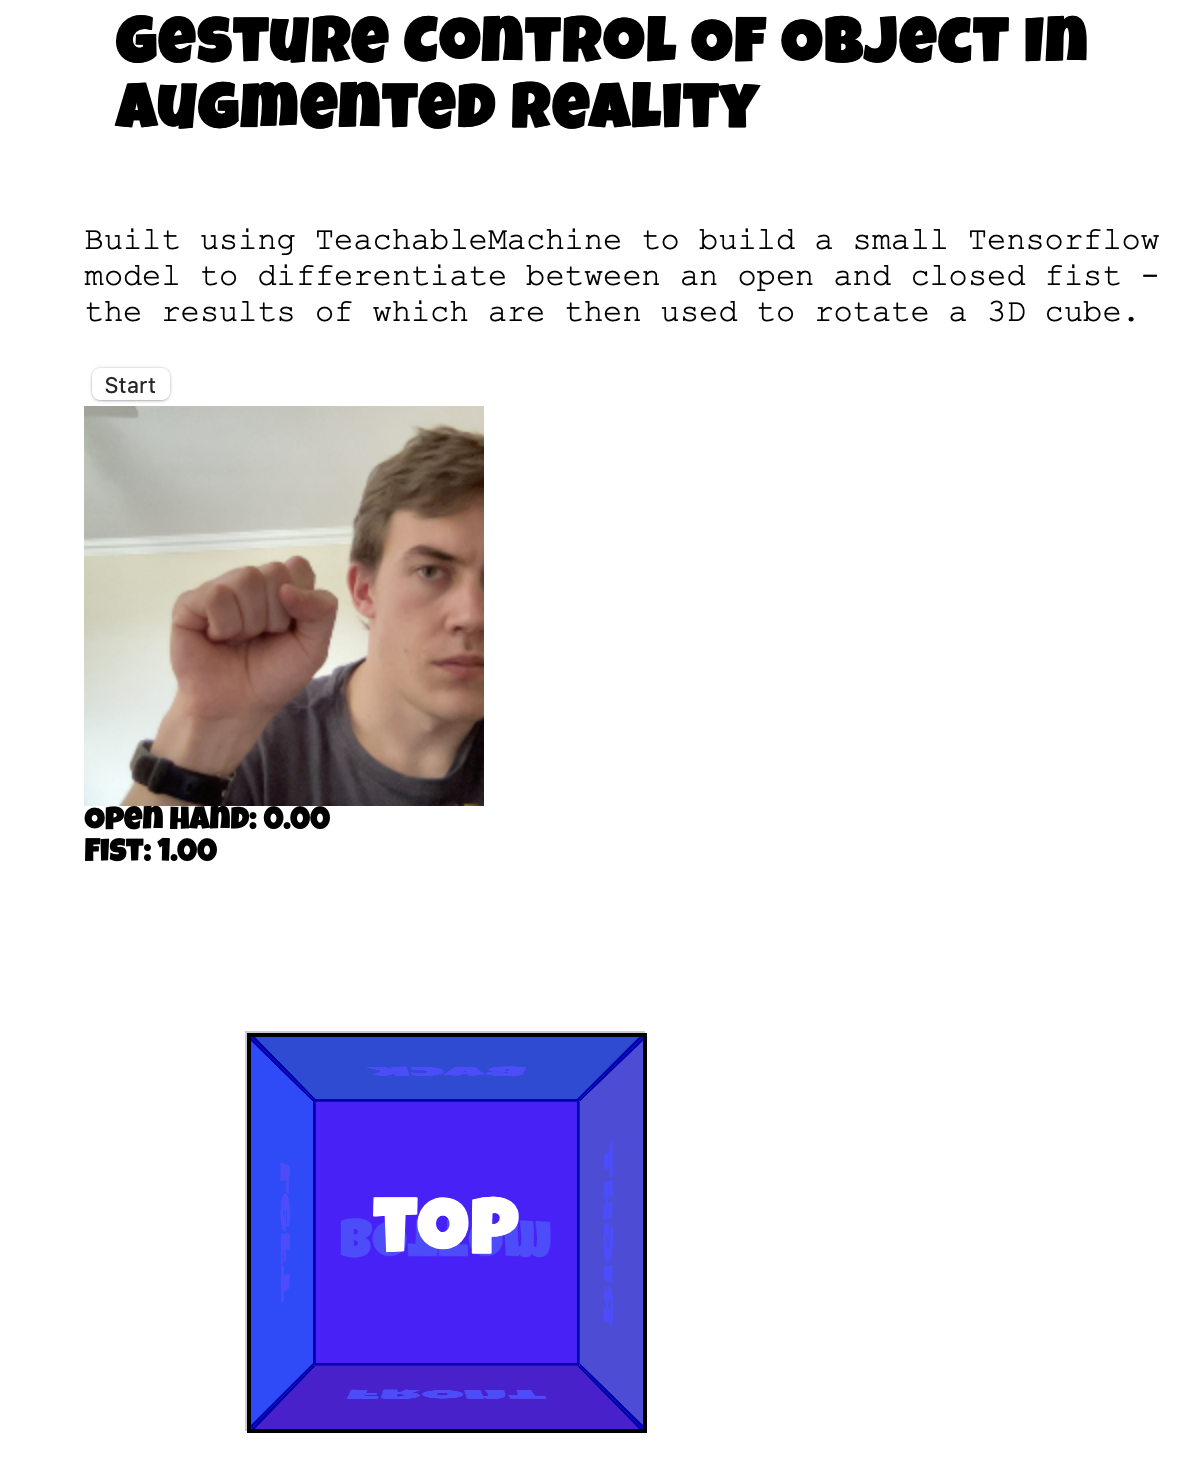
\includegraphics[width=0.4\linewidth]{figures/teachable_machine_2.png}
    \caption{Closed-hand input to TeachableMachine gesture recognition prototype}
    \label{fig:teachablemachine2}
\end{figure}

The rendering of a three-dimensional cube or similar object will require drawing over each frame of video. Representing each pixel of an image in a three-dimensional array of width x height x pixel values will allow each pixel to be changed as needed when a virtual object is "inserted" into the video. Using Python and the Pillow image library to convert an image into this array format, a simple prototype was built to render a three-dimensional cube onto a picture of a room. \FigRef{fig:room_cube} shows the output of this algorithm which just draws a small green cube over a random area of the image. Scaling this up to redrawing the cube for each frame of video and a different size and perspective based on the movement of the camera from the initial placement of the object seems feasible. \newline

\begin{figure}[!ht]
  \centering
  \includegraphics[width=0.8\linewidth]{figures/room_cube.png}
  \caption{Cube rendering prototype output}
  \label{fig:room_cube}
\end{figure}

The use of graphical libraries like \href{https://www.opengl.org}{OpenGL} or engines like the \href{https://unity.com}{Unity Engine} seems to be the industry standard for generating computer graphics and considering this is a critical element of the system it will probably need to be done partly off-the-shelf in order to generate realistic virtual objects. Rendering the virtual object as was done manually by replacing pixels in the cube rendering prototype seems inefficient and is predicted to not scale up well to the 24fps rendering needed for the final system. The creation of shadows on the environment is usually the next step in creating realistic lifelike objects but prototyping this needs to wait for depth information to be considered before it can be mapped onto the environment. \newline

\section[2022/04/03]{Sunday, 03 April 2022}

\subsection{Functional block diagram updates}

Time was spent refactoring the functional block diagram for the project proposal, splitting the system into four main processing components - the gesture recognition algorithm, the virtual object control algorithm, the environment recognition algorithm and the augmented reality creation. The second draft of the diagram can be seen in \FigRef{fig:fbd_draft2}. More detailed breakdowns are possible but this presents a high-level overview of the system and takes the approach of building a detailed skeletal model of the user's hand and a detailed depth map of the environment in which to place the virtual object. The Virtual Object Control subsystem was implemented as a template-matching system due to the constraints of memory and the advantage of being able to precompute and store certain gestures as templates for later use and identification. \newline

\begin{figure}[h]
    \centering
    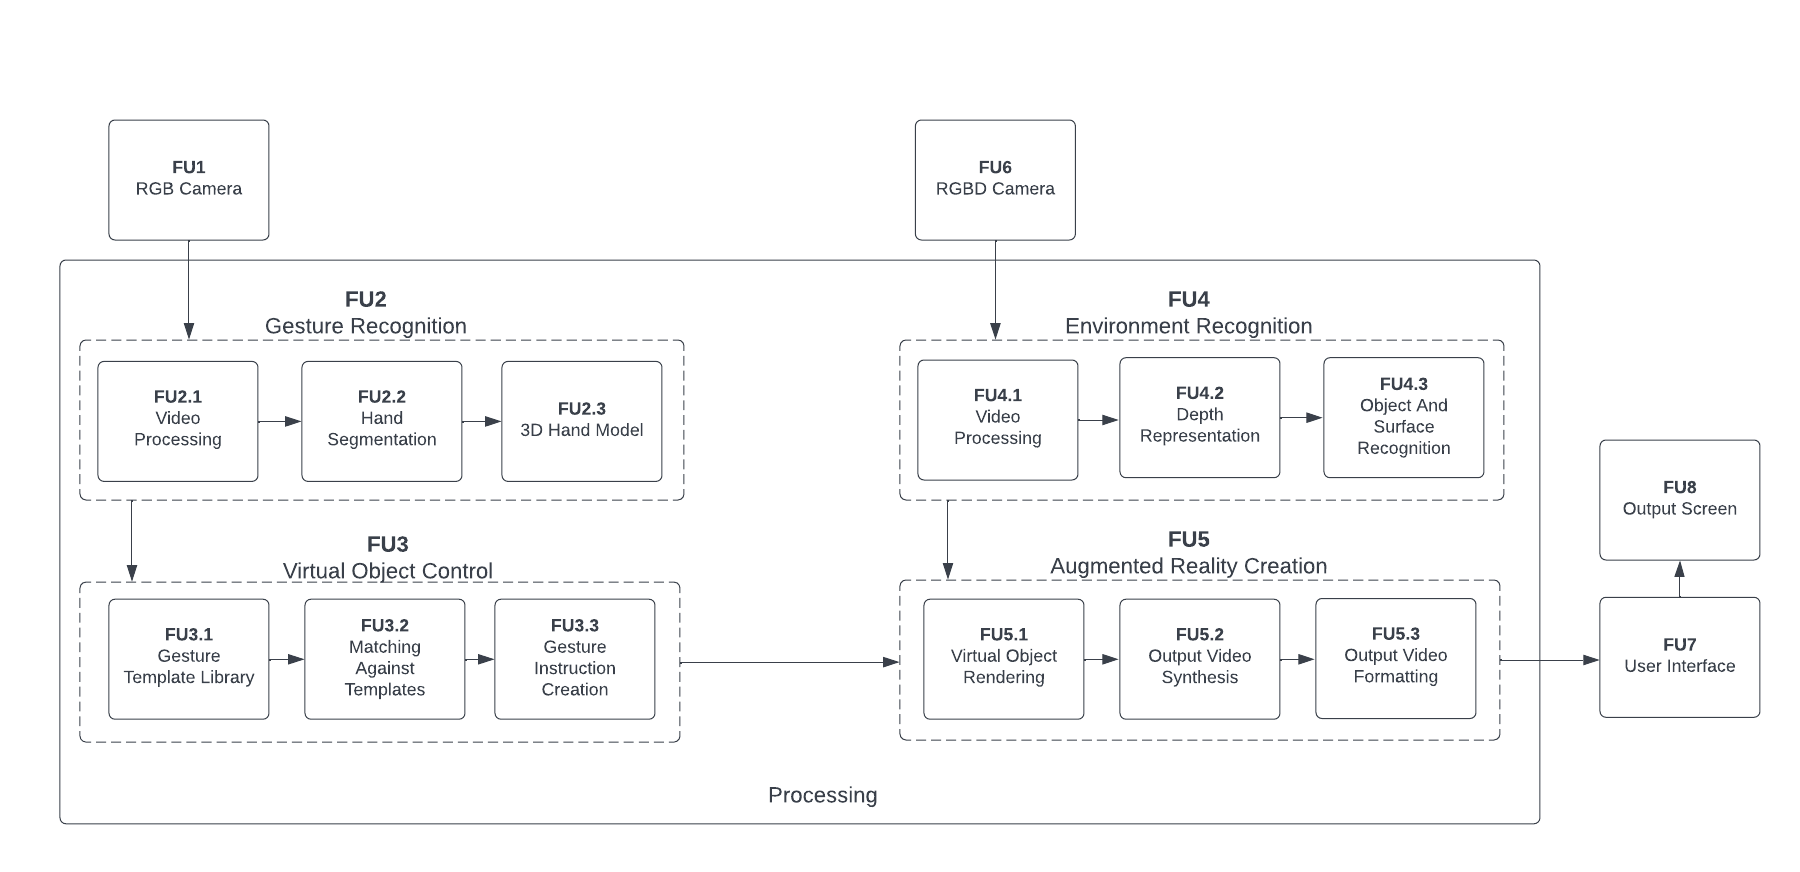
\includegraphics[width=1\linewidth]{figures/Functional Block Diagram_draft2.png}
    \caption{FBD draft 2}
    \label{fig:fbd_draft2}
\end{figure}

\subsection{Initial hardware prototypes}

In order to gain familiarity with ultrasonic sensors and depth measurement systems that might be needed to accurately map the environment around the system, a prototype was built using an HC-SR04 ultrasonic distance sensor with an Arduino Uno. The sensor was pointed around a roughly 4x4 metre room and different measurements taken to see if a small sensor like this could be used to generate a depth point cloud of an environment. The HC-SR04 ultrasonic sensor is a hobbyist sensor that has a maximum range of 4m and sends out a 40kHz sound wave out of an ultrasound transmitter and then receives any reflected sound waves on its ultrasound receiver. The time difference between sending out a sound wave and receiving one back can be used with the speed of sound in air (343m/s) to calculate the distance between the sensor and an object. \FigRef{fig:ultrasonic_setup} shows the ultrasonic sensor connected to the Arduino Uno and \FigRef{fig:ultrasonic_measuring} shows how a whiteboard was used to reflect the transmitted sound waves back at the sensor from varying distances. These distances were steadily increased from an initial 4cm as the whiteboard was moved further away from the sensor and a graph of these results is provided in \FigRef{fig:HCSR04_graph}. \newline

\begin{figure}[h]
    \centering
    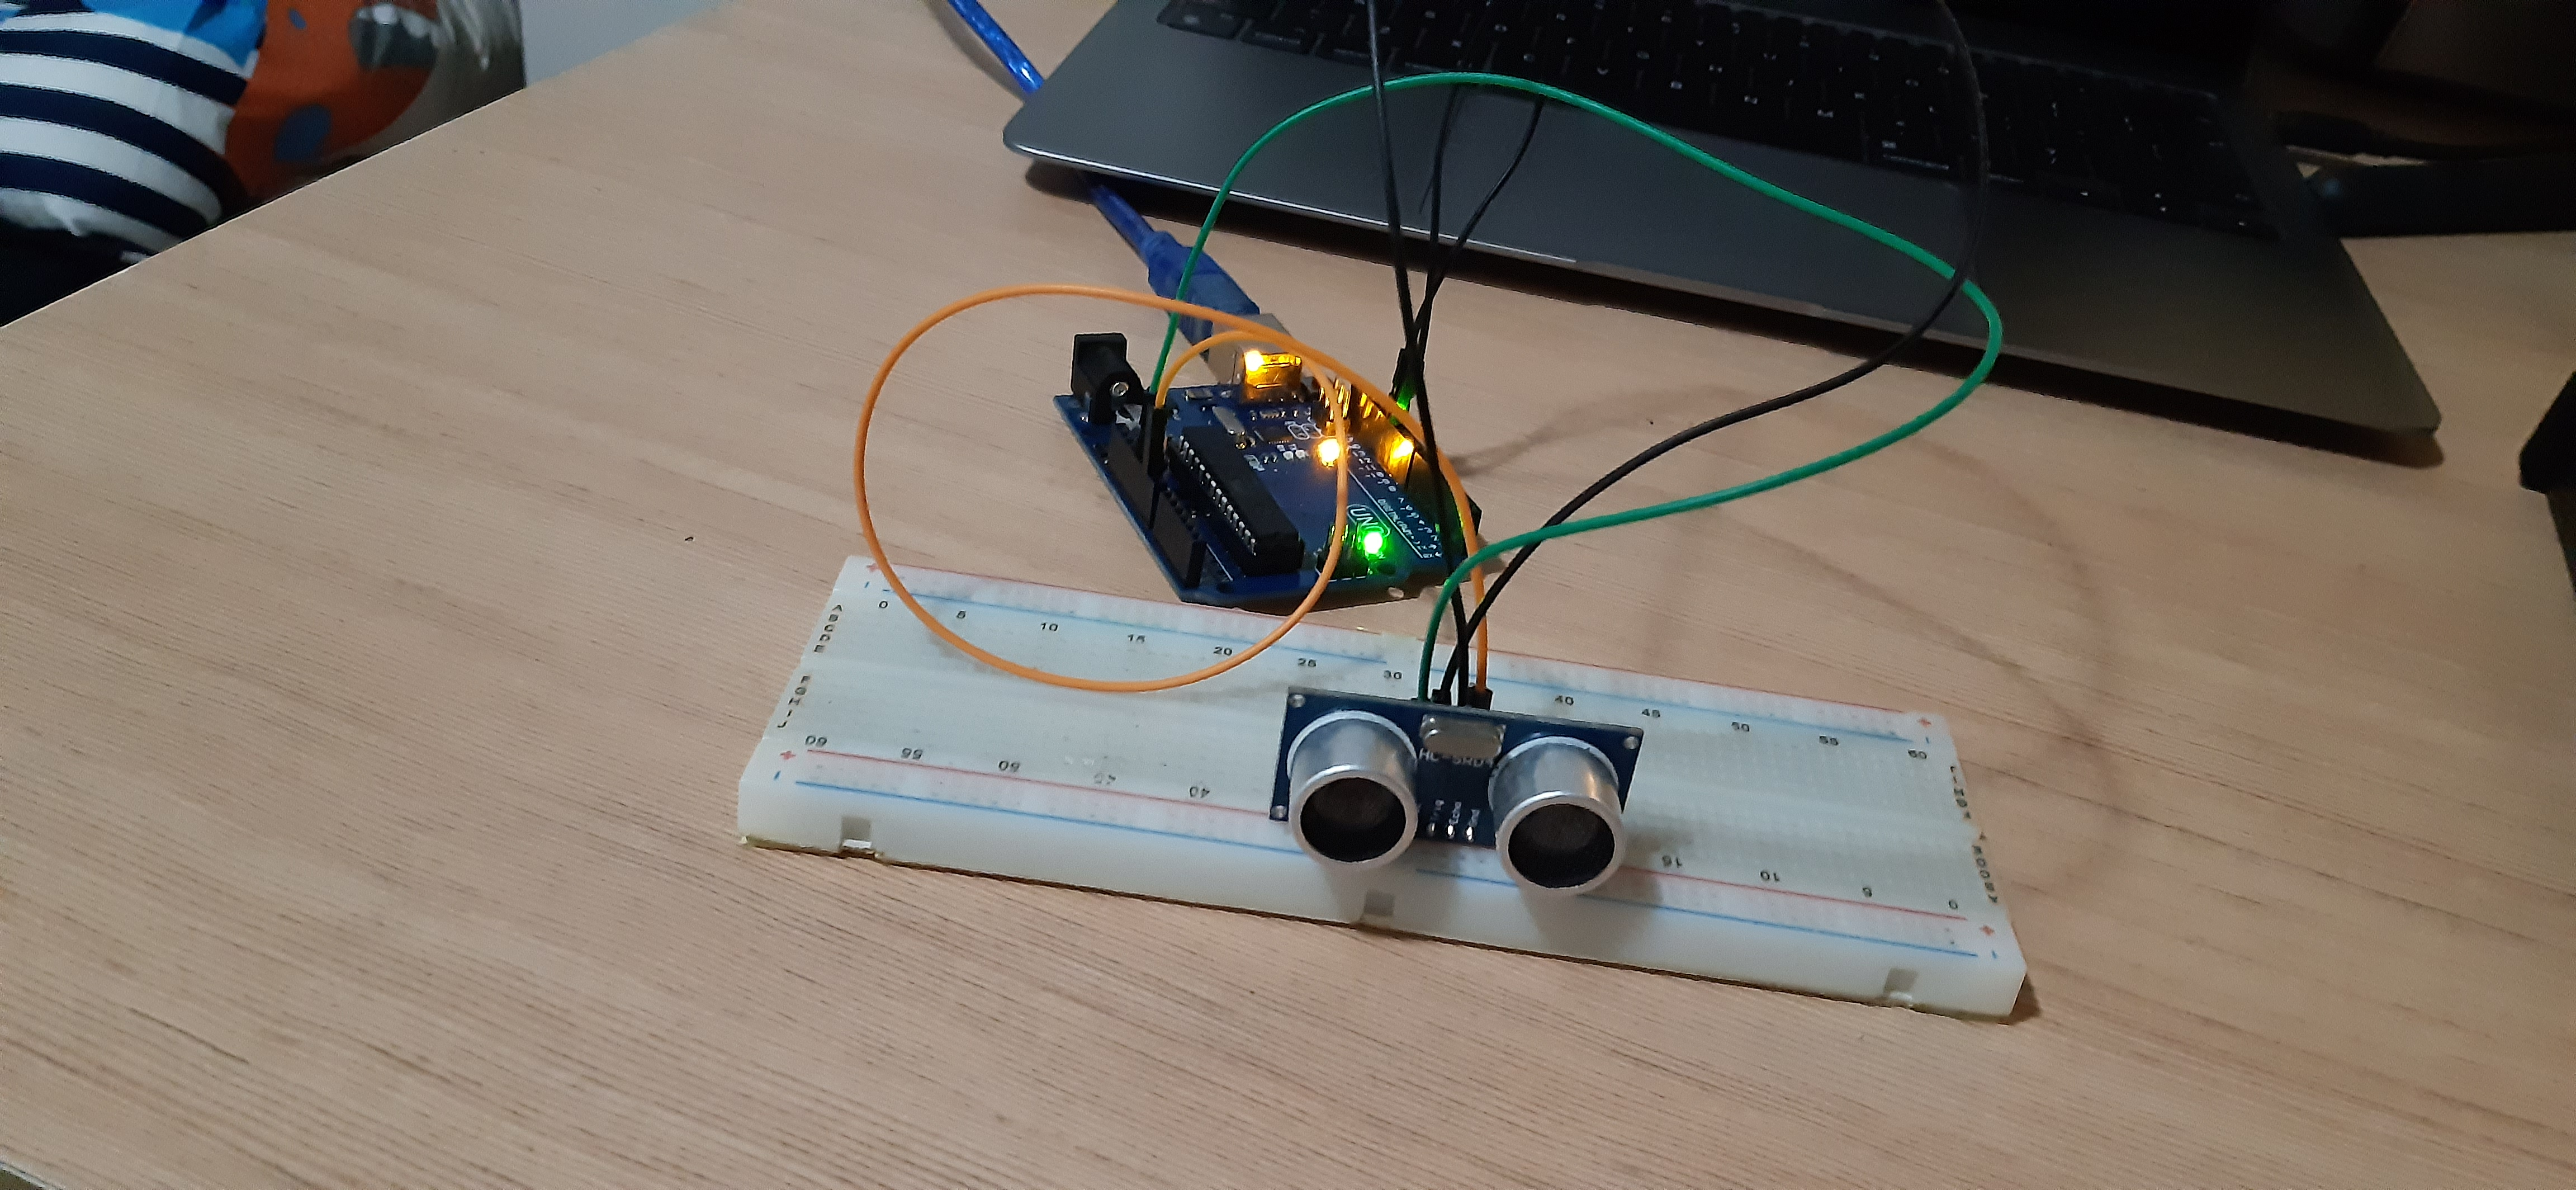
\includegraphics[width=0.5\linewidth]{figures/ultrasonic_prototype_setup2.jpg}
    \caption{The ultrasonic sensor connected to an Arduino Uno}
    \label{fig:ultrasonic_setup}
\end{figure}

\begin{figure}[h]
    \centering
    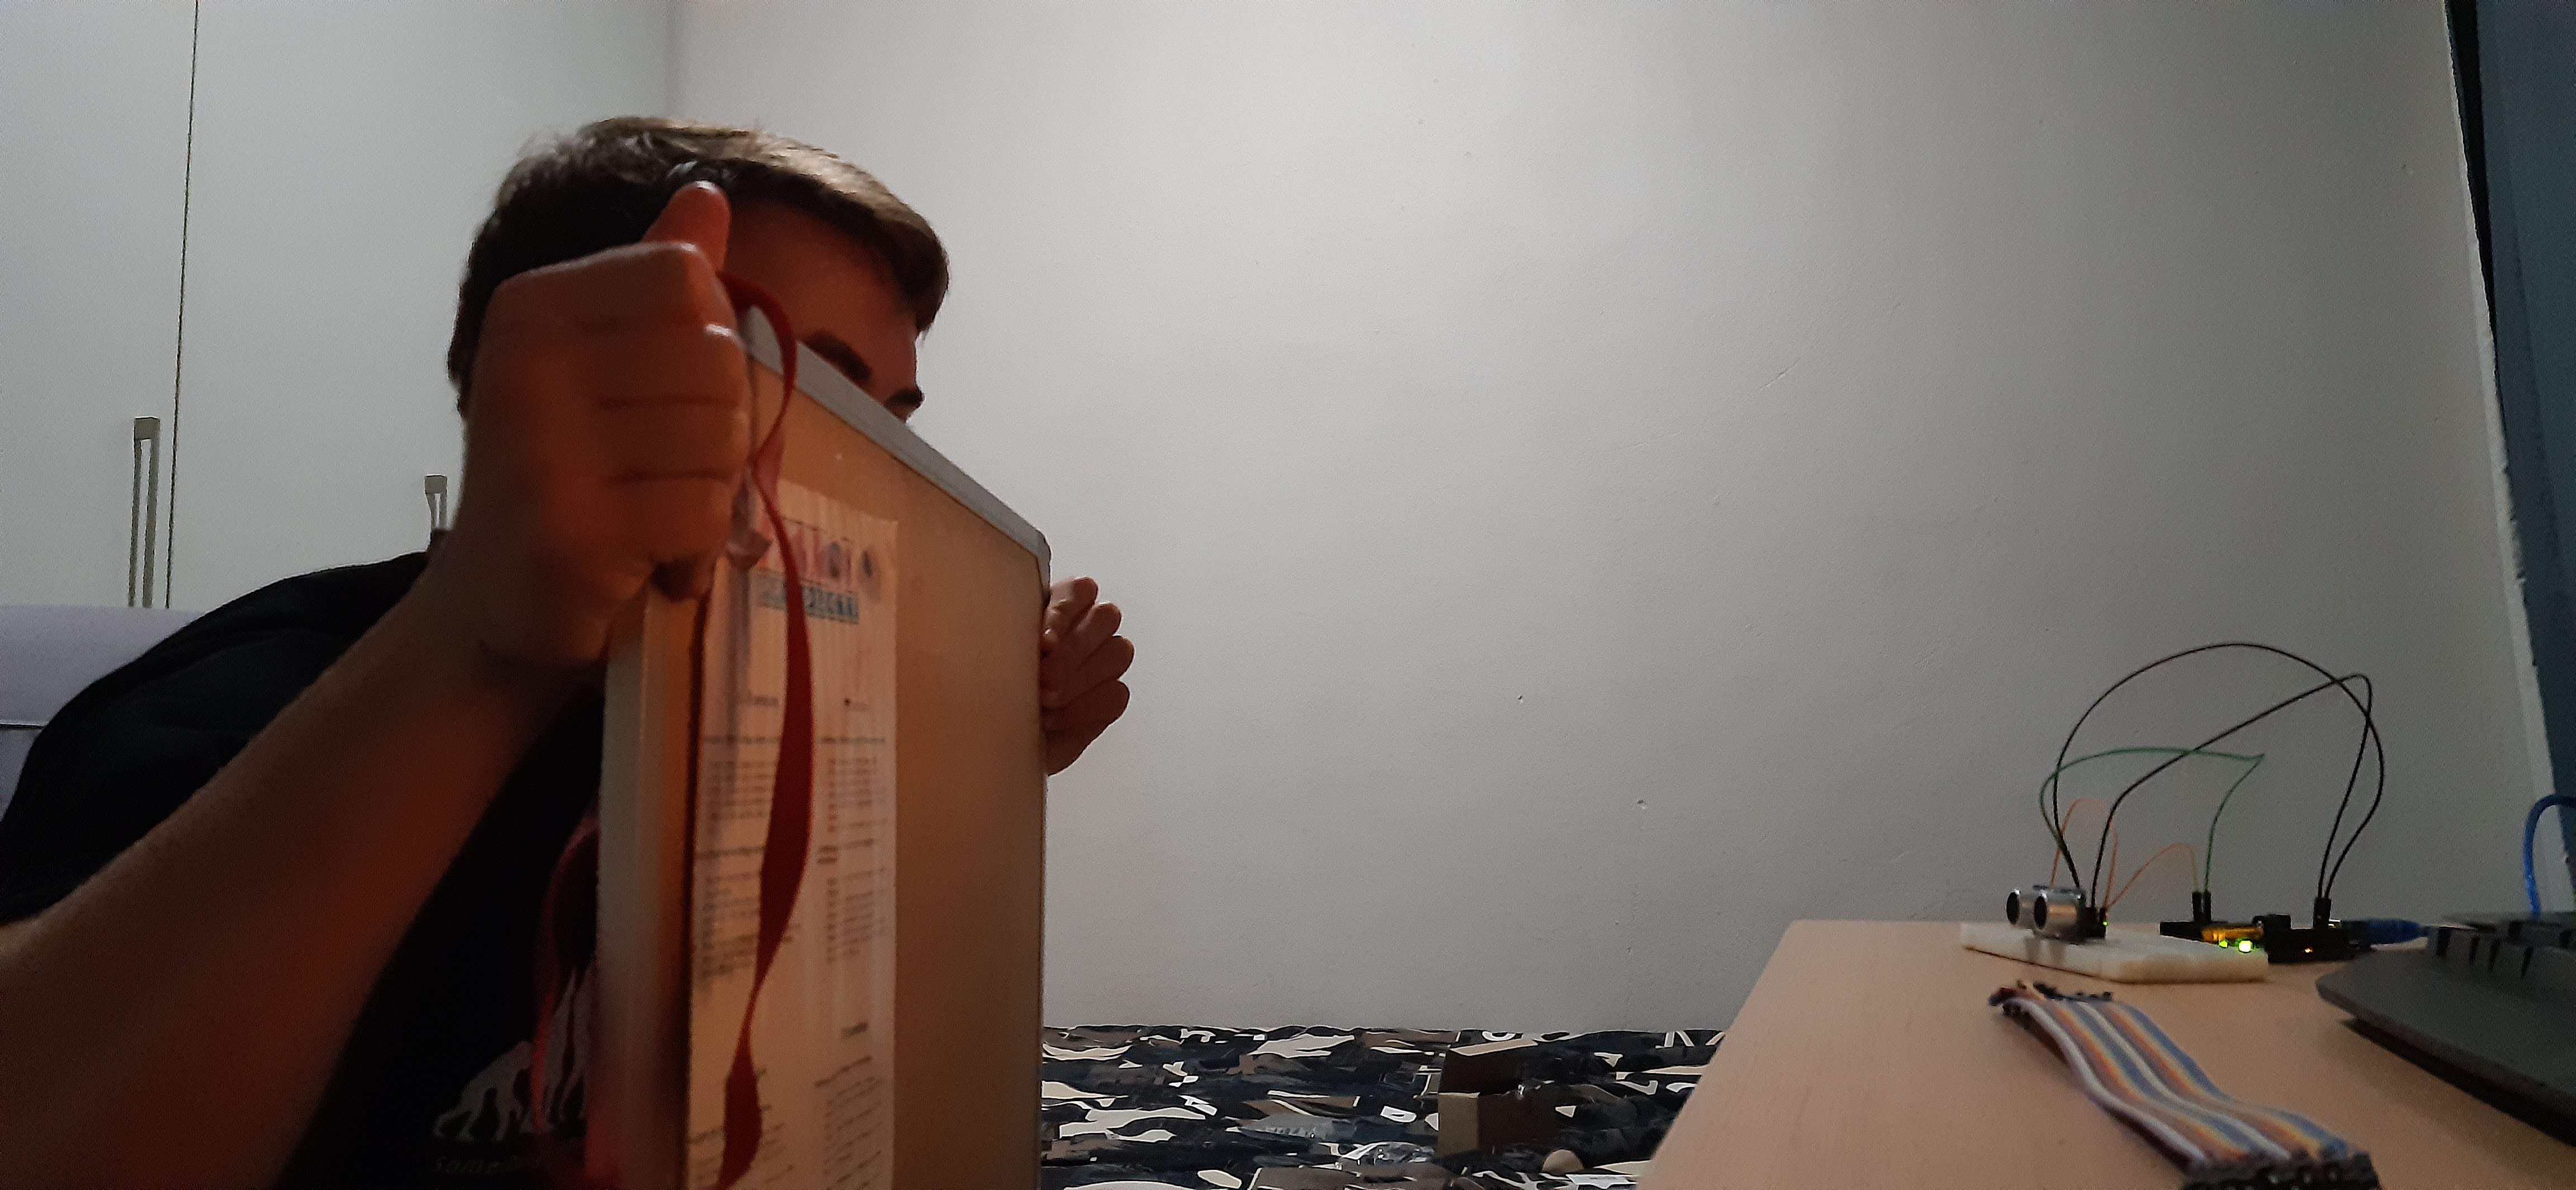
\includegraphics[width=0.5\linewidth]{figures/ultrasonic_prototype_setup1.jpg}
    \caption{The ultrasonic sensor measuring test}
    \label{fig:ultrasonic_measuring}
\end{figure}

\begin{figure}[h]
    \centering
    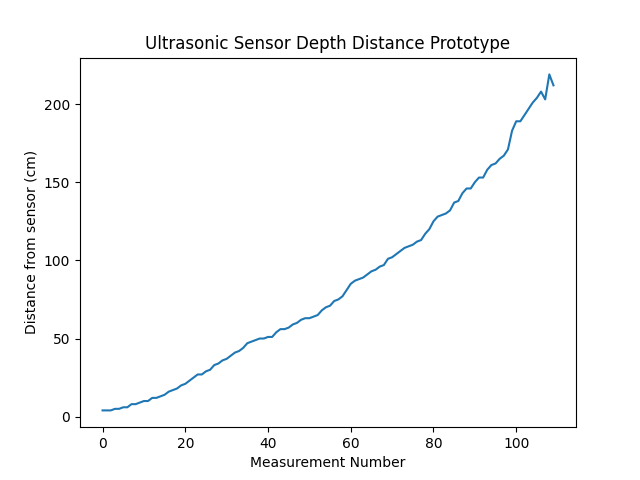
\includegraphics[width=0.4\linewidth]{figures/ultrasonic_prototype_graph.png}
    \caption{Graph of measuring experiment using HC-SR04}
    \label{fig:HCSR04_graph}
\end{figure}

The measurements became too noisy to be useful past 2m but the sensor performed well before this. However, it is noted that the sensor did not reliably pick up reflected sound waves reflected by a person or other soft objects like pillows and this is theorized to be due to the shallow effectual angle of less than 15$\deg$ for the receiver - irregular shapes like human body parts did not reflect the sound wave straight back at the receiver and thus didn't create any input. This is a problem for a virtual object system that must be able to visualize the surrounding environment accurately so that objects can be placed in it and interact correctly with hard and soft objects alike. Similarly, the ultrasonic sensor only projects sound waves in a straight line and thus has a narrow field of vision that limits the depth-sensing range of the device to an almost flat plane in space. This is not adequate for fully mapping an environment around the system and thus a more robust depth-mapping solution like a spinning platform with an ultrasonic sensor on it, LIDAR sensor or Microsoft Kinect's light-emitting depth measurements needs to be considered. \newline

\section[2022/04/04]{Monday, 04 April 2022}

\subsection{Project proposal improvements}

Time was spent refactoring the project proposal according to Mr. Grobler's comments and completing additional sections. The skeletal hand model was decided upon as the method for determining hand gestures because it has the most fine-grained information for different gestures and can be implemented using an RGB camera only as opposed to requiring depth information. The skeletal model developed by Zhang et al. \cite{mediapipe_hands} serves as inspiration as to what can be accomplished using off-the-shelf components such as \href{https://www.tensorflow.org}{Tensorflow}. The system developed by Zhang et al. was optimized for mobile use using TensorflowLite but still performed best in a desktop application runtime. Thus, this behaviour in addition to numerous other papers implementing gesture control on PCs only leads to the conclusion that the system should be implemented on a PC and not an embedded platform. This is in addition to the graphical demands of creating a virtual object and handling the input of two separate cameras - a task that demands either a very expensive embedded platform that is beyond the budget of this system or a PC. \newline

The system requirements were developed for the project proposal based on the research presented above in this lab book. Additionally, \href{https://www.redsharknews.com/technology-computing/item/3881-why-24-frames-per-second-is-still-the-gold-standard-for-film}{RedShark Cinematography} explains that 24fps is the standard frame rate for movies because it is slow enough for the human eye to fill in missing frames and create a moving picture in the brain but fast enough to not appear janky or disjointed - the way silent films of the 1920s appeared due to hand-cranked film cameras. Thus 24fps is the minimum frame rate decided upon for updating of the virtual object and hand model. \newline

The field specifications were similarly designed in addition to the University of Warwick's \href{https://warwick.ac.uk/services/healthsafetywellbeing/guidance/officelighting/}{Lighting Guidance For Offices} which states that standard office lighting for computer work should be 300lux. The 2m distance of the virtual object to the RGBD camera comes from the ultrasonic test prototype in which sensor output became too noisy after 2m of distance between the sensor and reflecting object and dimensions of most offices. \newline

\section[2022/04/05]{Tuesday, 05 April 2022}

\subsection{Embedded neural network prototype}

The final prototype to be built from the list written on the 31st of March was "A small image recognition system that could identify at least 1 distinct hand gesture on a small embedded platform like an ESP32." This was implemented by using an off-the-shelf ESP32 Cam example Arduino file that downloads and runs inference on a TensorflowLite Model. The model created previously using TeachableMachine in the Hand Gesture Web demo was used again and loaded onto the device. \FigRef{fig:esp32_cam1} and \FigRef{fig:esp32_cam2} show the results of the model when an open palm and fist are displayed to the camera of the ESP32. The model does not accurately differentiate between the two different gestures shown to it and this is theorized to be because of minimal training data that was all webcam input and now this low-resolution camera input is not matching to any of the expected inputs to the neural network. \newline

Additionally, the model is incredibly slow and can interpret the hand gestures nowhere near 24 times a second - it is estimated generously that it is making a prediction once every second. The ESP32 cam also does not record video at a high-enough resolution to capture hand features well enough that a 21-point skeleton could be modelled. Thus the results of this prototype point towards a much higher resolution camera being needed to provide input for the gesture recognition system as well as more processing power and better training for the computer vision algorithm that is ultimately implemented for the hand gesture recognition. \newline

\begin{figure}[h]
    \centering
    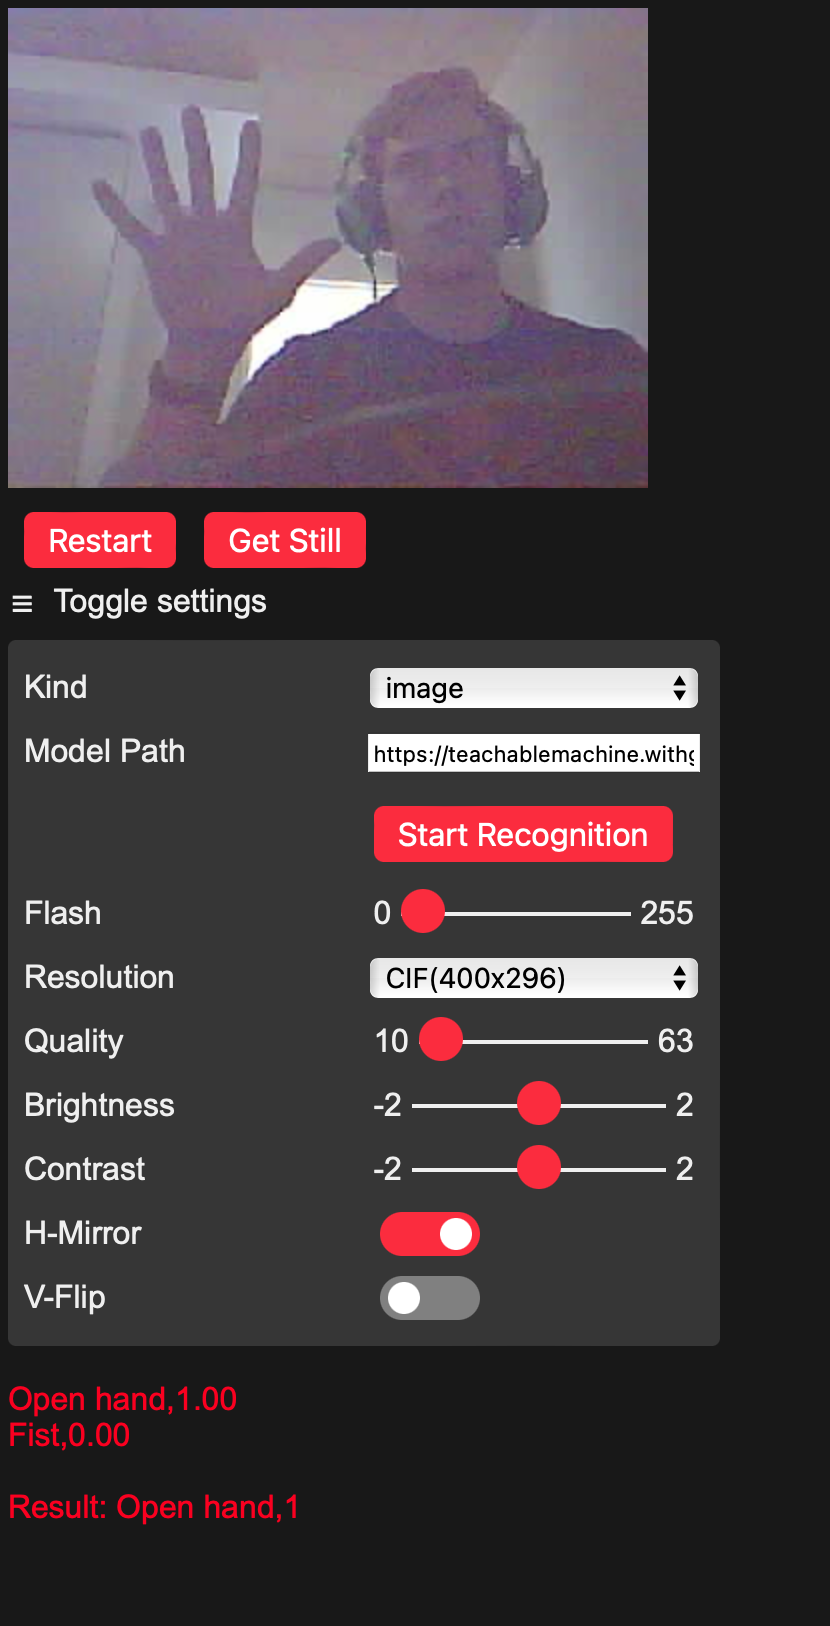
\includegraphics[width=0.3\linewidth]{figures/esp32_cam_open.png}
    \caption{Output of the ESP32 web server running the hand gesture model}
    \label{fig:esp32_cam1}
\end{figure}

\begin{figure}[h]
    \centering
    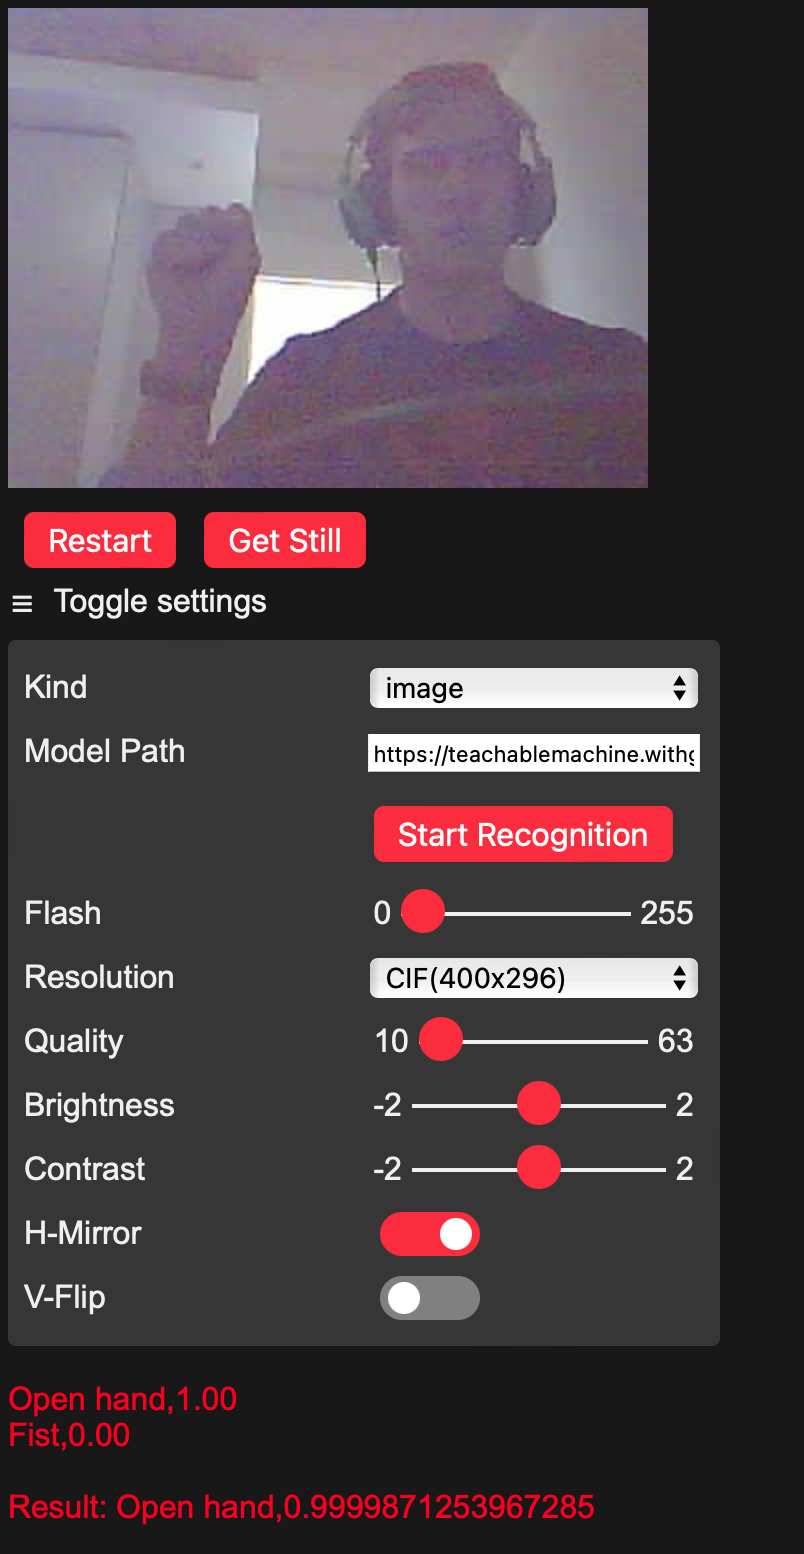
\includegraphics[width=0.3\linewidth]{figures/esp32_cam_fist.png}
    \caption{Output of the ESP32 web server running the hand gesture model}
    \label{fig:esp32_cam2}
\end{figure}

\section[2022/04/14]{Thursday, 14 April 2022}

\subsection{Libfreenect demonstration program}

Some changes were made to the project proposal today in order to converge upon a third draft of the proposal. However, the salient discovery of the day was discovering the \href{https://github.com/OpenKinect/libfreenect}{Libfreenect} open source library that makes controlling a Microsoft Kinect possible on both Windows, Mac and Linux. Two Microsoft Kinect devices were signed out from Mr. Grobler's hardware store last week and this library appears to contain the drivers necessary to interface with the Kinect on modern PC platforms. \newline

Testing with the library needs to be conducted but it appears wrappers for the API in Python, C, Java and C++ are all available. The choice of programming language will obviously be decided by engineering factors such as the required speed of the system and graphical library support. However, it is predicted that if real time speed is becoming difficult to achieve that C might be needed for its low-level high-performance nature but if Python can provide adequate performance it may be much more utilitarian and conducive to constructing the more complicated parts of the project such as matrix mathematics and 3D scene reconstruction with point clouds. This informs the direction in which to take the design of following prototypes.\newline 

\section[2022/04/15]{Friday, 15 April 2022}

\subsection{Libfreenect testing}

The libfreenect library was installed and the demo program that comes with the installation was used to pull basic information from one of the Microsoft Kinects - a RGB image was displayed from the camera and a false color image with different colors representing different depth measurements from the depth camera. A screenshot of this demo running on an Apple Macbook Air M1 is displayed in \FigRef{fig:kinect_demo}. However although the demonstration program runs adequately on this machine, installing the library in the Python environment of the laptop proved difficult and ran into many compiler errors since libfreenect is a C library re-optimized for use with Python and the environment of the laptop proved difficult to set up. This installation troubleshooting is still ongoing. \newline

\begin{figure}[h]
    \centering
    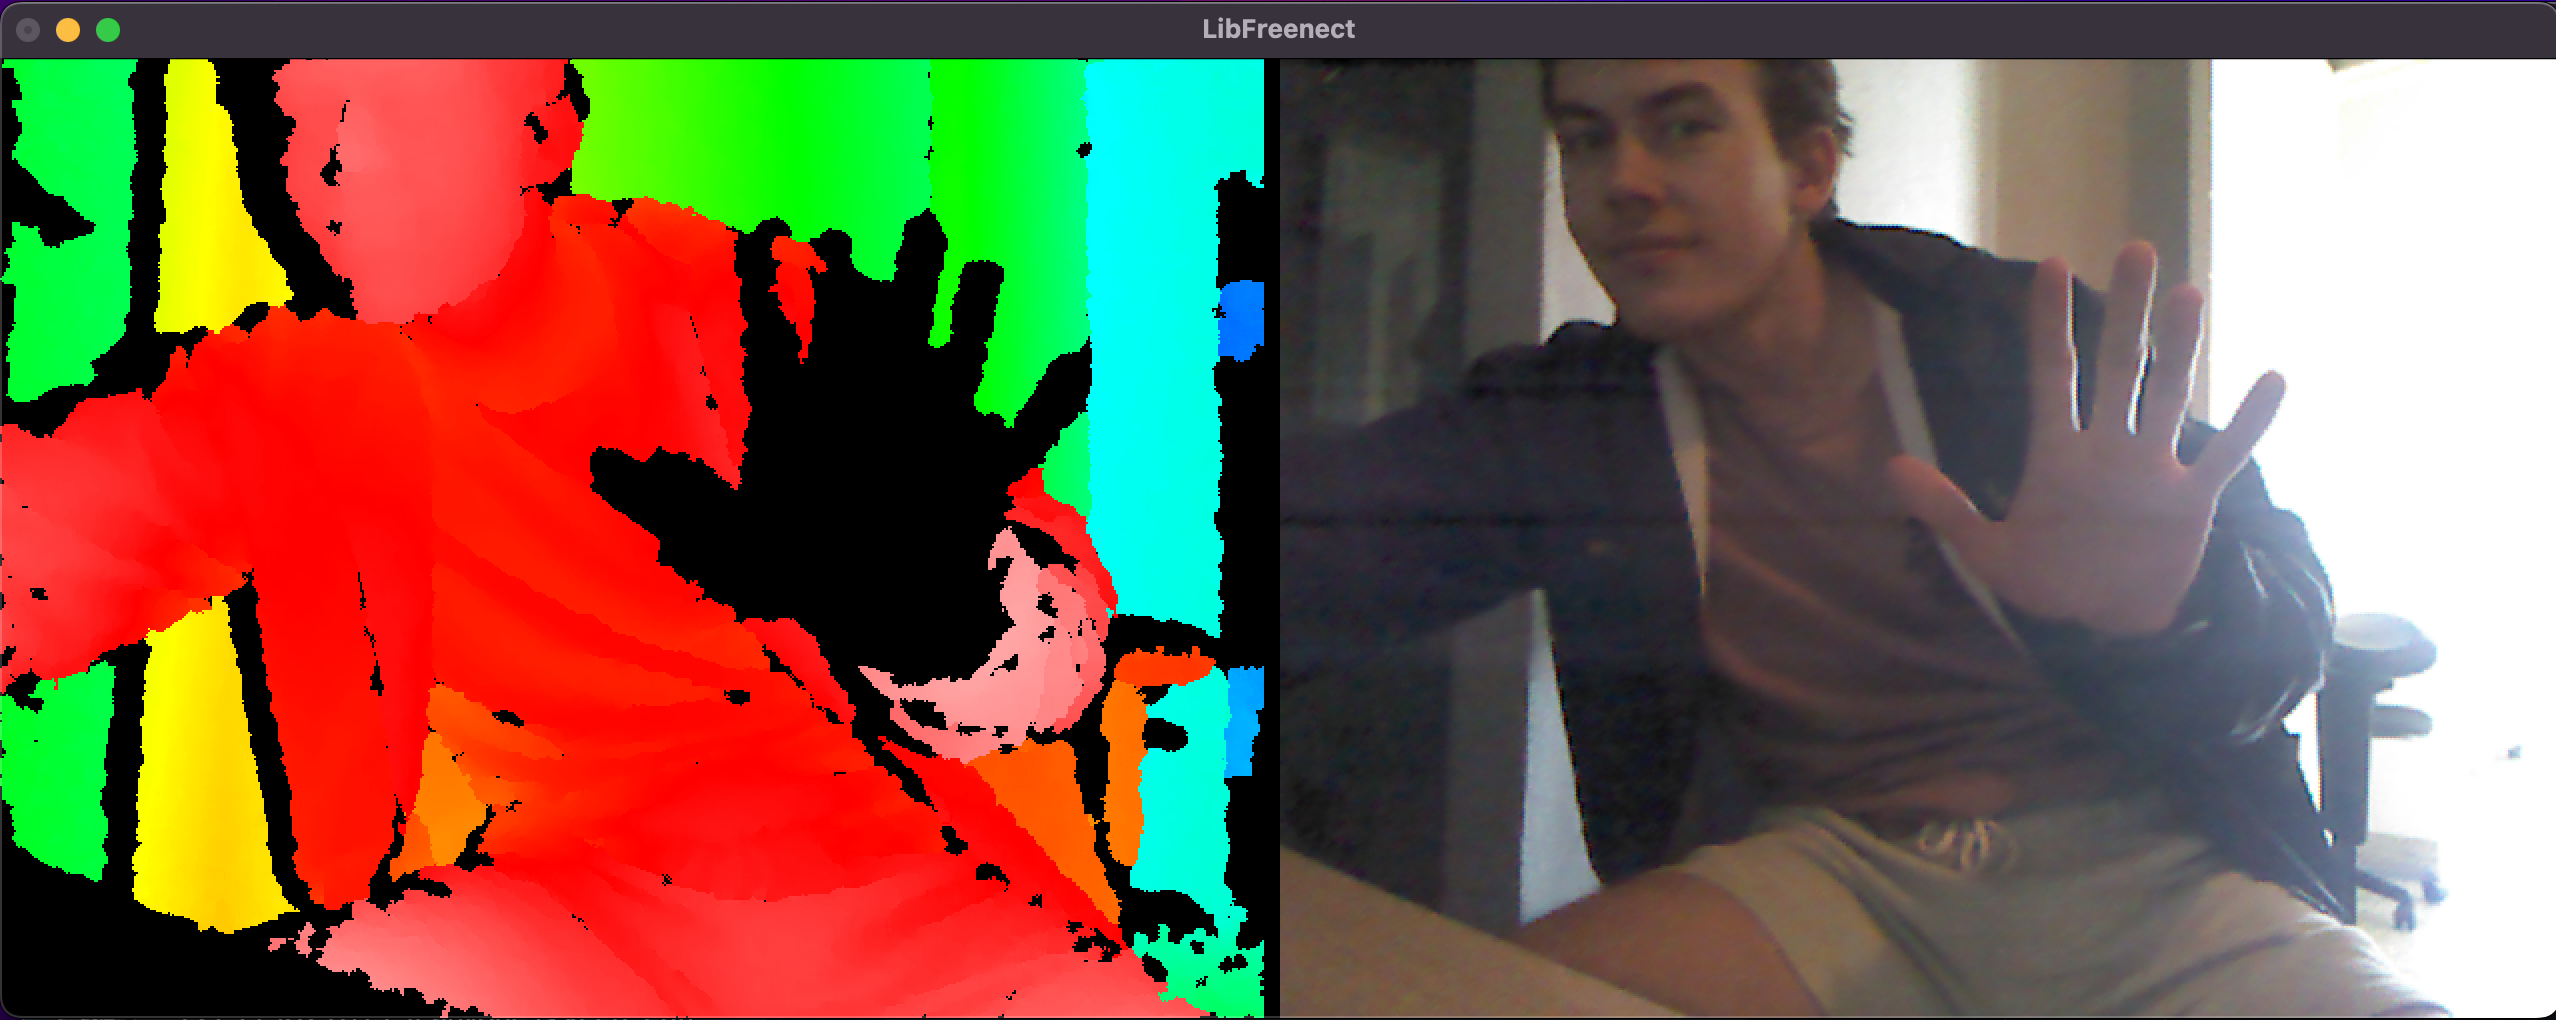
\includegraphics[width=0.8\linewidth]{figures/kinect_demo.png}
    \caption{Output of the libfreenect demo program}
    \label{fig:kinect_demo}
\end{figure}

\section[2022/04/20]{Wednesday, 20 April 2022}

\subsection{Initial Version Of Experimental Plan}

\textbf{Qualification Test 1: Observation Of Result Of Manipulation Of Virtual Object Using Single Hand Gestures}

Objective: To confirm the user can manipulate a virtual object using the discrete gestures of a single hand.
 
Equipment Used: The two input cameras, a ruler and a PC are used.

Experimental Parameters and setup: The two cameras are connected to the PC and the system initialized. The front-facing camera is pointed directly at the user and the rear-facing camera is pointed at the environment directly in front of the user and PC with a big enough flat surface visible so that the virtual object is instantiated onto it. A list of the expected behaviours of the virtual object for the various gesture inputs is generated for comparison against.

Experimental Protocol: The user will hold up their hand and display each discrete hand gesture for controlling the virtual object for two seconds each. These gestures are those for the up, down, left, right, rotate on the x-axis, rotate on the y-axis, rotate on the z-axis, backwards and forwards commands for the virtual object. The observed change in the virtual object will be noted, and its distance moved on the flat surface measured with a ruler. These measurements will be noted against the expected behaviour for these gesture commands.

\textbf{Qualification Test 2: System Recognition Confirmation Of Hand Gestures In Real Time}

Objective: To ensure that the individual hand gestures can be recognized by the system in the time required to ensure that the system operates in user-apparent real-time and that the known gestures of the system can be accessed in the same required time period.

Equipment Used: The two input cameras, a PC and a software timer will be used.

Experimental Parameters and setup: The system hardware will setup and initialized as for Qualification Test 1 and then a software timer added to the code to measure the time between a new frame of video being received by the system to the time a gesture prediction is returned by the system.

Experimental Protocol: The user displays the 9 different gestures for various commands to the virtual object. As this is done the system logs how long each prediction of which gesture is being displayed takes to generate and writes these values to a log file. This generation process checks the current hand gesture against known gestures in memory and returns the predicted gesture. Ensuring that the correct gesture is recognized for each, the software timer logs are examined, and each comparison time ensured to be less than 41.6ms so that the system is recognizing the user's hand gestures at a user-apparent real-time of 24fps.

\textbf{Qualification Test 3: Testing The System's Physically Accurate Rendering Of A Virtual Object}

Objective: To ensure that the system can accurately model a three-dimensional object in augmented reality.

Equipment Used: The two input cameras, a PC, a screenshot tool and a physical 20cm by 20cm cube will be used.

Experimental Parameters and setup: The cameras are setup and the system initialized as in Qualification Test 1. A physical 20cm by 20cm cube is placed onto the flat surface in front of the rear-facing camera.

Experimental Protocol: The physical cube will be moved ten centimeters in each direction and rotated 180 degrees in each planar direction. After each movement a screenshot of the rear-facing input video feed will be taken to acquire a reference image of the physical cube. Then, the gesture instructions for each virtual object control command will be sent to the virtual object control algorithm manually and a screenshot will be taken of the output video feed of the virtual object in the environment. The two sets of screenshots will be compared to ensure that the virtual cube is accurately modelled in augmented reality in reference to the real-world cube.

\textbf{Qualification Test 4: Frame Rate Measurement And Real-Time Operation Of The System}

Objective: To ensure that the system is updated in real-time and displays output video that appears to have no visible latency to the user.

Equipment Used: The two input cameras and the first-principles frame counter will be used.

Experimental Parameters and setup: The input cameras are setup as for Qualification Test 1 and the frame counter displayed on the user interface.

Experimental Protocol: The user will display the 9 hand gestures for the various commands to the virtual object for 2 seconds each and the frame counters for the virtual object rendering algorithm as well as the hand model creation algorithm will be observed - if they stay above 24fps the system is operating with a latency less than 41.6ms and will appear to run instantaneously to the user in real-time.

\textbf{Qualification Test 6: Confirming Physical Realism Of Virtual Object Behaviour}

Objective: To ensure that the virtual object behaves in the physically realistic manner in which a real object would behave.

Equipment Used: The two input cameras, a PC, a timer, a ruler and a physical 20cm by 20cm cube will be used.

Experimental Parameters and setup: The two input cameras are setup as for Qualification Test 1 and the physical cube will be placed on a flat surface in front of the rear-facing camera.

Experimental Protocol: The system will be initialized so that the virtual cube object appears on the flat surface and no input commands will be provided to the system. The virtual cube should remain stationary on the flat surface for 10 seconds before the user attempts to move (using gesture control) the object past the right of the physical cube first with 30cm of distance between the virtual cube and the physical cube, then 20cm, 10cm and 0cm. This process is then repeated for the left, right, backwards and forwards commands with the physical cube being moved to the position where it stands in the path of the virtual object. The virtual object's position should be noted at each attempted movement and its movement observed - the virtual object will only be able to move past the physical object when 10cm or more space exists between them, measured by the ruler.

\section[2022/04/30]{Saturday, 30 April 2022}

\subsection{Image thresholding prototypes}

The aim of the work session today is to experiment with thresholding, image segmentation and image processing to estimate what kind of methods will be needed for the final system to function and effectively derive information from a webcam and convert that into gesture input. To that aim, the OpenCV and PIL libraries were installed onto a PC and a Python program implemented. This program converted a webcam image into an array of pixel values and then scanned through all the columns and rows of the array pixel by pixel and evaluated if the three RGB pixels were close to the RGB values of the colour red. If they were, the algorithm left them be else the pixel was set to white and the algoirthm proceeded to the next pixels. \\

In this way, a red thresholding algorithm was implemented and attempted to pull out just the parts of the webcam image that were red. Red was chosen in this case because it is a striking color and none of the background items at the time contained much red in them, while the foreground item - a person wearing a red hoodie did. The results of the algorithm are presented below in \FigRef{fig:red_thresholder_original} and \FigRef{fig:red_thresholder_test}. It is clear that the shadows and shades of the red hoodie make it difficult to get an accurate thresholded shape and comparing pixels on an individual basis misses a lot of what is actually trying to be thresholded. Considering pixels and the average of a few pixels is predicted to be a better method of doing this with a kernel-based approach. But even so, the color-based thresholding is not suitable for the hand segmentation approach as people's hands are all different colors and different parts of the body have the same color. Thresholding with a grayscale image and specific hand segmentation approaches will next be investigated. Greyscale images are where the value of a pixel merely represents the amount of light present in that pixel and is often used to separate background and foreground information because background pixels are usually less intense than foreground images which are closer to a camera

\begin{figure}[h]
    \centering
    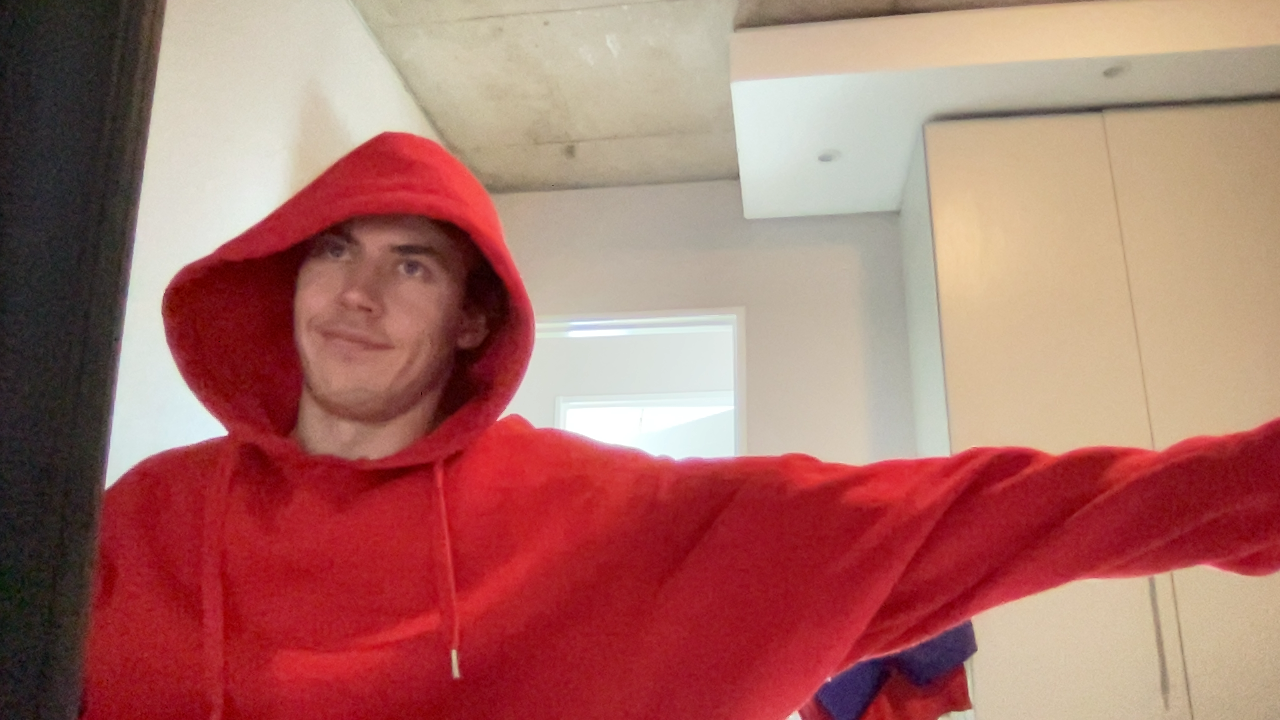
\includegraphics[width=0.4\linewidth]{figures/red_thresholder_original.png}
    \caption{Webcam input to the red thresholder algorithm}
    \label{fig:red_thresholder_original}
\end{figure}

\begin{figure}[h]
    \centering
    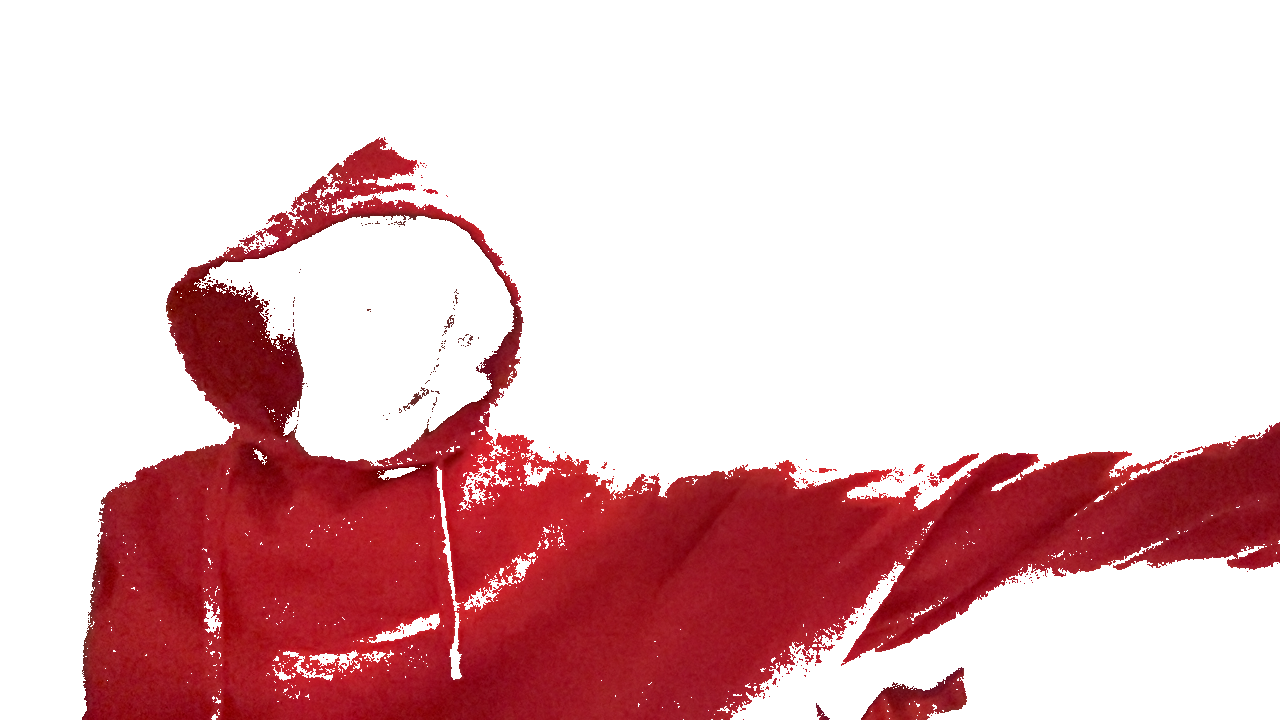
\includegraphics[width=0.4\linewidth]{figures/red_thresholder_test.png}
    \caption{Output of the red thresholder algorithm}
    \label{fig:red_thresholder_test}
\end{figure}

A greyscale thresholding implementation is now tested. The image is converted to grayscale and five different threshold algorithms used - these are the binary, inverted binary, truncated, truncated to zero and truncated to zero inverted thresholding functions. The results of these implementations are visible in \FigRef{fig:threshold_binary} to \FigRef{fig:threshold_zero_inverse}. The inverse binary threshold algorithm performs the best in terms of delineating a human form from background imagerey. These tests were performed in a relatively dark room and environmental factors are to be considered when implementing a thresholder that must function in various lighting conditions.

\begin{figure}[h]
    \centering
    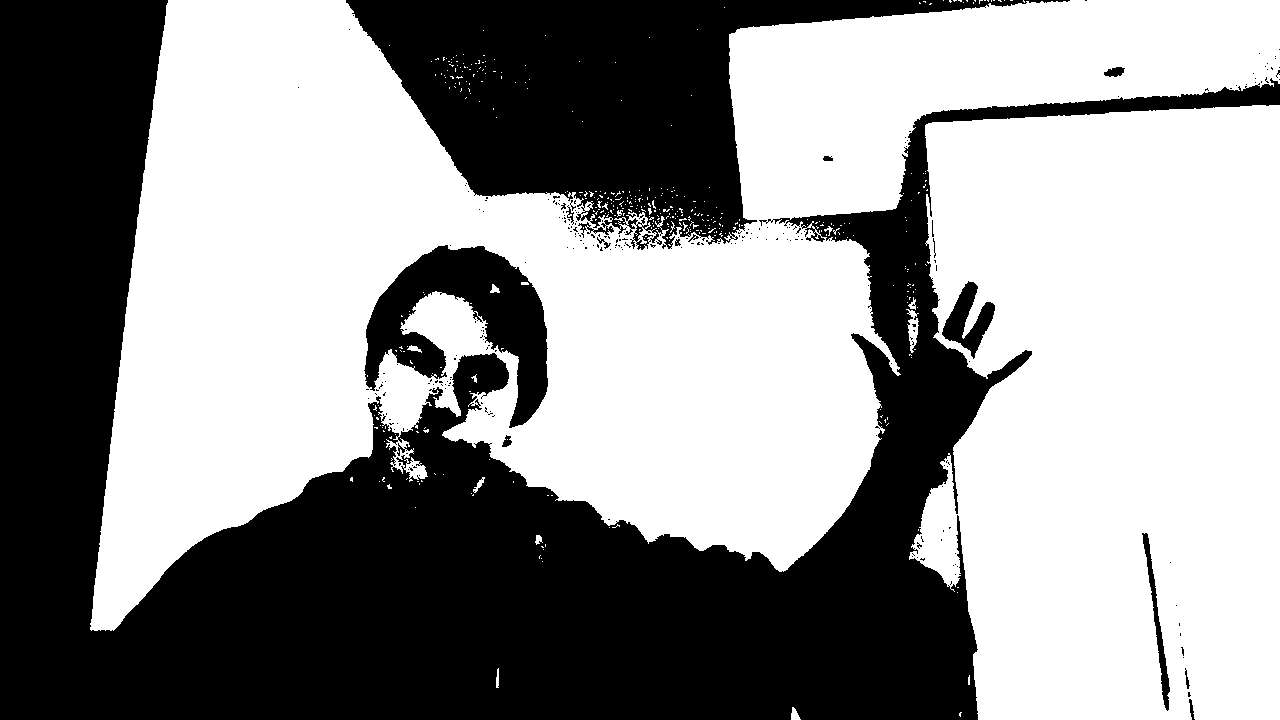
\includegraphics[width=0.4\linewidth]{figures/threshold_binary.png}
    \caption{Binary threshold algorithm}
    \label{fig:threshold_binary}
\end{figure}

\begin{figure}[h]
    \centering
    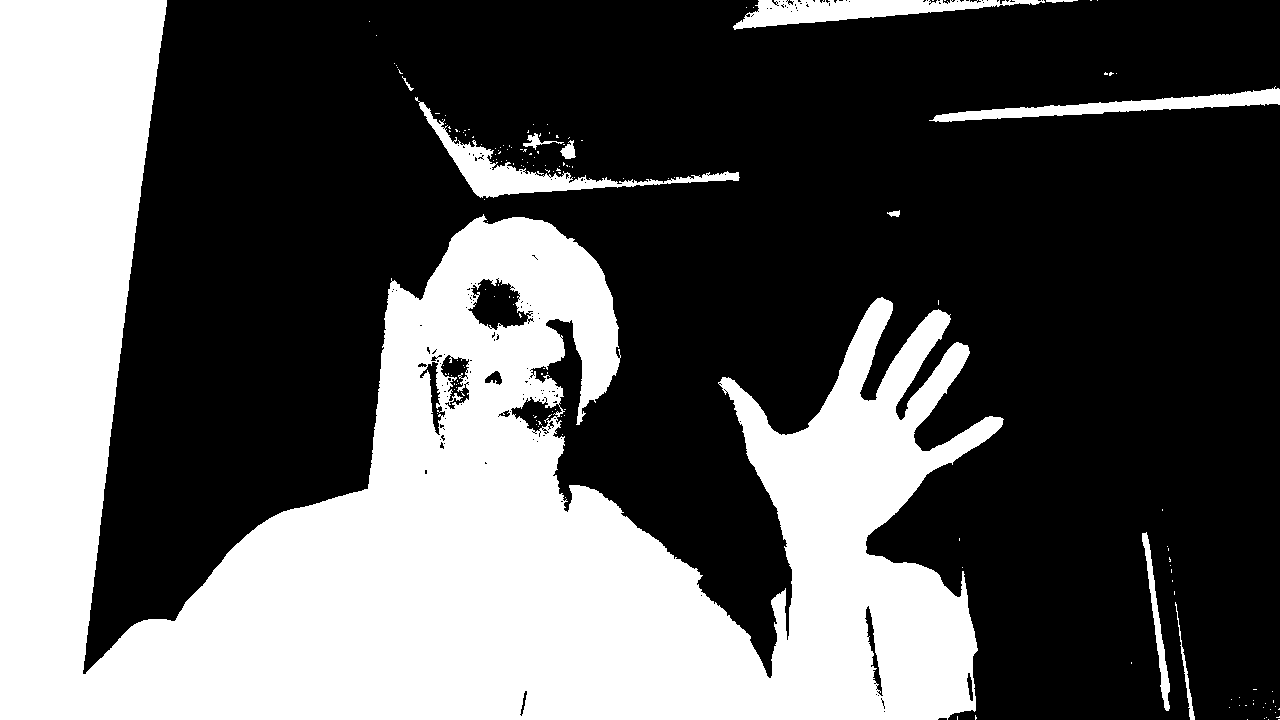
\includegraphics[width=0.4\linewidth]{figures/threshold_binary_inverse.png}
    \caption{Inverse Binary threshold algorithm}
    \label{fig:threshold_binary_inverse}
\end{figure}

\begin{figure}[h]
    \centering
    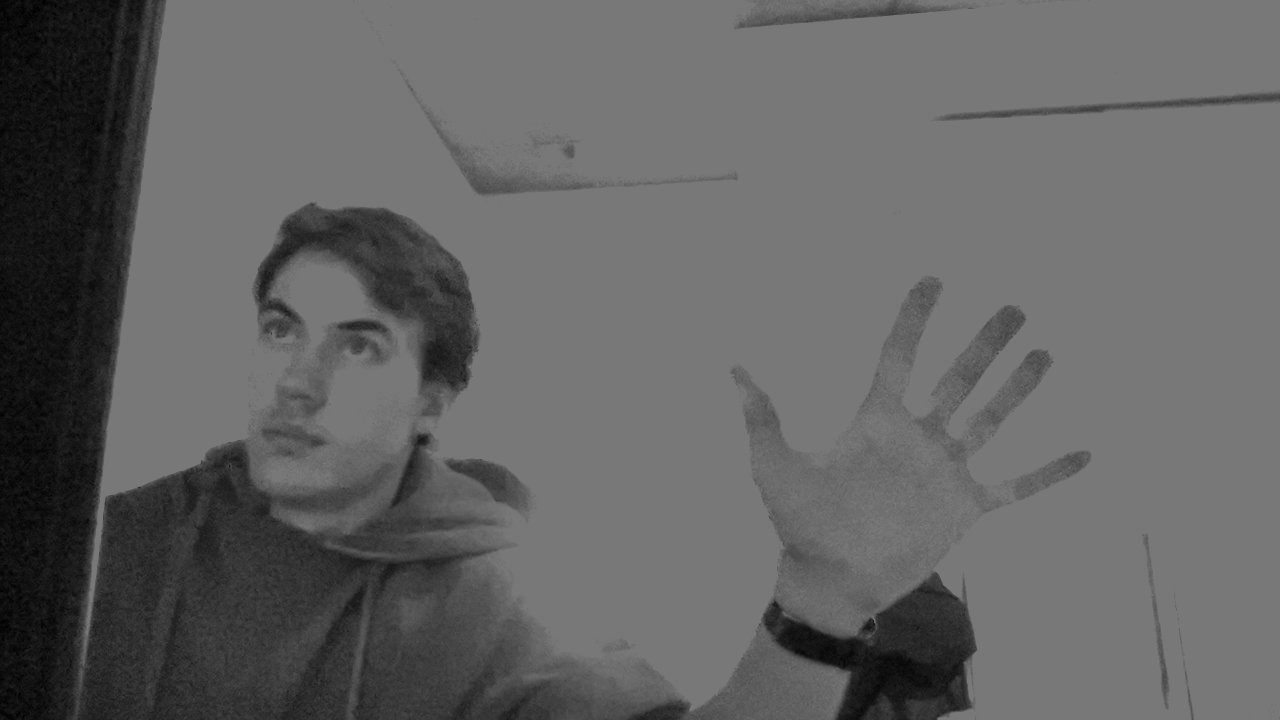
\includegraphics[width=0.4\linewidth]{figures/threshold_truncated.png}
    \caption{Trucated threshold algorithm}
    \label{fig:threshold_truncated}
\end{figure}

\begin{figure}[h]
    \centering
    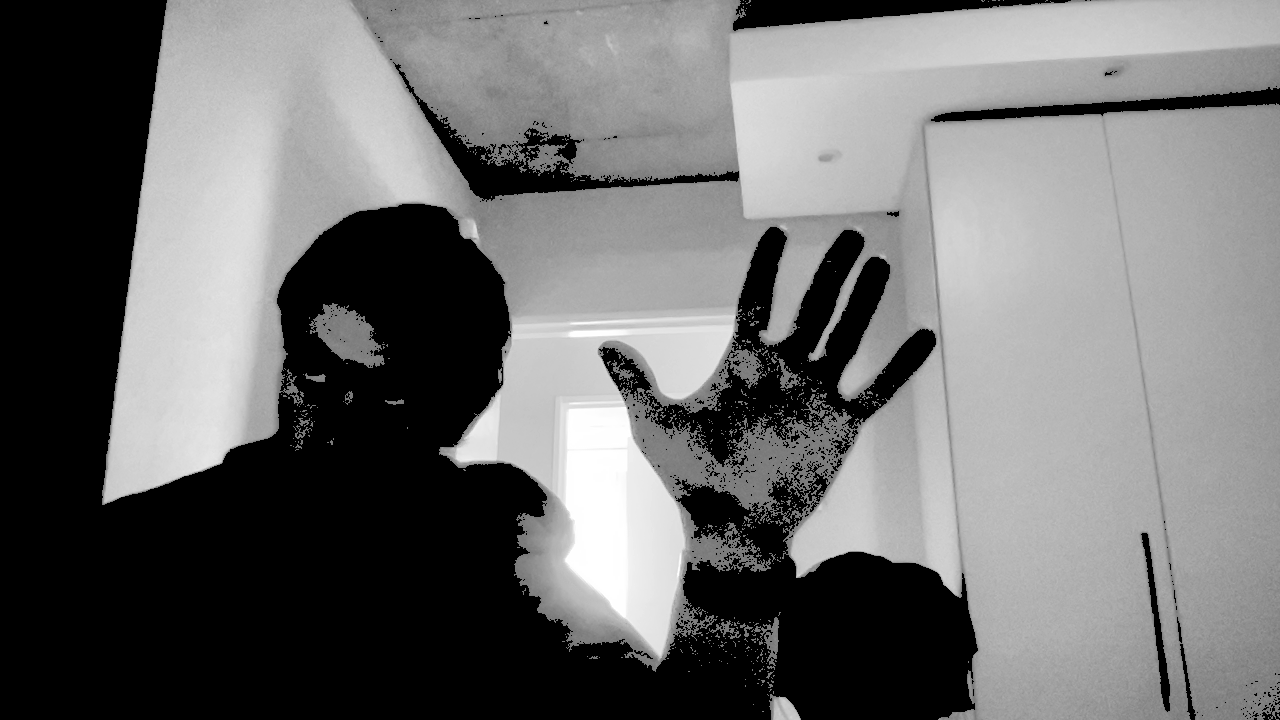
\includegraphics[width=0.4\linewidth]{figures/threshold_zero.png}
    \caption{Truncated Zero threshold algorithm}
    \label{fig:threshold_zero}
\end{figure}

\begin{figure}[h]
    \centering
    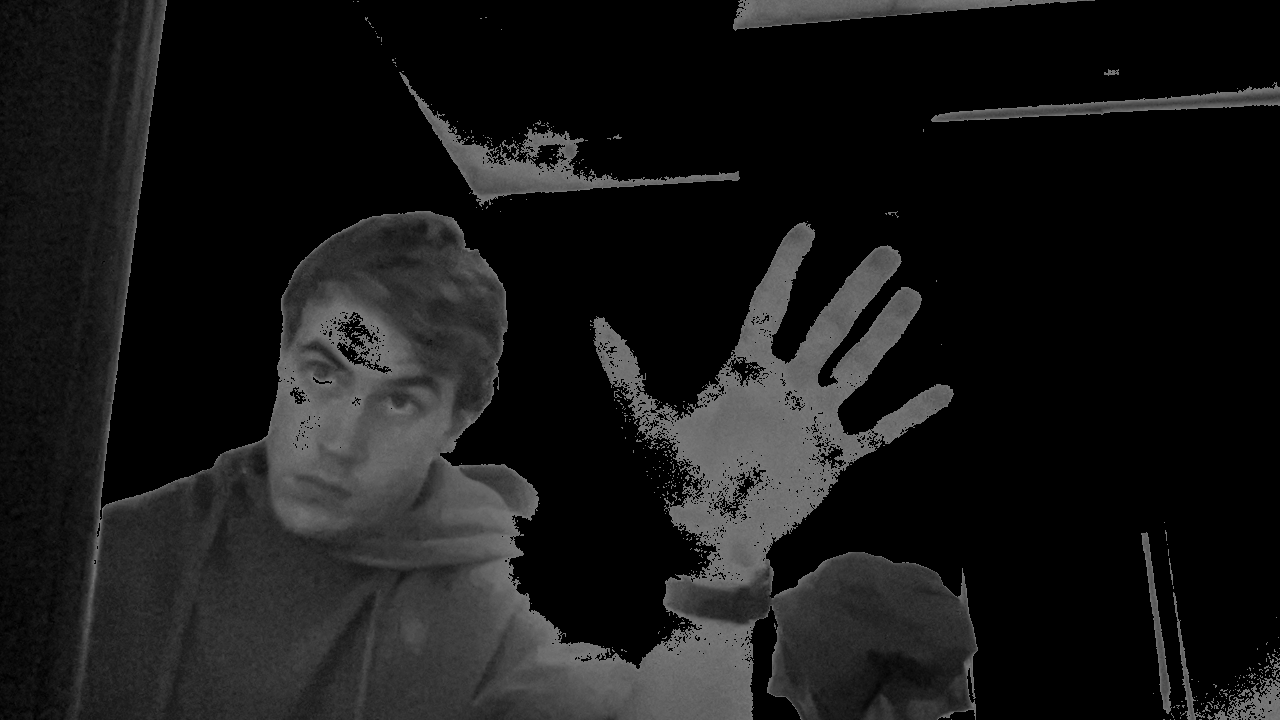
\includegraphics[width=0.4\linewidth]{figures/threshold_zero_inverse.png}
    \caption{Inverse Truncated Zero threshold algorithm}
    \label{fig:threshold_zero_inverse}
\end{figure}